\documentclass[a4paper]{jsarticle}
  \usepackage[T1]{fontenc}
\usepackage{lmodern}
%
\usepackage{amsmath}
\usepackage{amssymb}
\usepackage{bm}
\usepackage[dvipdfmx]{xcolor}
\usepackage[dvipdfmx]{graphicx}
\usepackage{tikz}
\usetikzlibrary{patterns}
\usepackage{ascmac}
\usepackage{multirow}
%
\usepackage{gfncmd}
\usetimessetMatrix
\makeparenwidthresized
%
\usepackage{gfnlf}
\let\limpleqv\iff
\useupperquantifierheight
\makeleftparenomittable{lflimpleqv}{existsin}
%
\usepackage{gfndecox}
\usepackage{gfndecox-std1}
\newnonumberdecoclass{\sublempar}{�����}{top}%(box�ɂ���ƕ������������Citembox �‹��� \textwidth �ɏ]���Ă��Ȃ��H)
%
\usepackage{gfncls}
\setsectiontheme{strongline}
%
\setlength{\parskip}{1em}

  \usepackage{style}
%
  \title{線型数理要論}
  \author{\texttt{@bd\string_gfngfn}}
\begin{document}
\maketitle
%
\section{はじめに}
  \subsection{概要}
    \plainpar{}{
      この文書では,あまり基底のとり方や線型写像といった一般の議論を意識せず,
      行列を単に「体 $K$ の元が $m \times n$ に並んだもの」として捉えてその性質を見ていく方針をとる.
    }
  \subsection{基本的定義}
    \defpar{}{
      非負整数を\newword{自然数}といい,自然数全体からなる集合を $\setN$,また正整数全体からなる集合を $\setNpos$ と書く.
      自然数 $n \in \setN$ に対し,
      $\Natleq{n} \defeq \setprnsep{k \in \setNpos}{k \leq n}$ とする.
    }
    \defpar{行列に関する記法}{
      体 $\seqprn{K, +, \cdot; 0, 1, \paren{\dummysign}^{-1}}$ の元を並べた
      $m \times n$ 行列全体からなる集合を $\setMatrix{m}{n}{K}$ と書く.
      行列 $A \in \setMatrix{m}{n}{K}$ の $\seqprn{i, j}$ 成分を $A_{i j}$,第 $j$ 列を $\colvec{A}{j}$ と書く.
      $A \in \setMatrix{m}{n}{K}$ に対し,各 $j \in \Natleq{n}$ に於いて
      \begin{align*}
        \colvec{B}{j} &\defeq
          \begin{cases}
            \vecb         &\caseif{j = k}\\
            \colvec{A}{j} &\caseow
          \end{cases}
      \end{align*}
      で定められる行列 $B \in \setMatrix{m}{n}{K}$,すなわち“$A$ の第 $k$ 列をベクトル $\vecb$ で上書きした行列”を
      $\coloverwrite{A}{k}{\vecb}$ と書く.
      また $A \in \setMatrix{m}{n}{K}$ と $I \subseteq \Natleq{m}$ に対して
      “$A$ のうち $I$ に属する行番号だけ取り出した $\card{I} \times n$ 行列”を $\rowsubmatrix{A}{I}$ と書き,
      $J \subseteq \Natleq{n}$ に対して
      “$A$ のうち $J$ に属する列番号だけ取り出した $m \times \card{J}$ 行列”を $\colsubmatrix{A}{J}$ と書く.
    }
\section{行列と行列式}
  \subsection{ブロック行列}
    \thmpar[thm:det-mult-homomorphism]{行列式演算と積の準同型性}{
      正方行列 $A, B \in \setMatrix{n}{n}{K}$ に対して
      \begin{align*}
        \det \paren{A B} = \det A \cdot \det B
      \end{align*}
      が成り立つ.
    }
    \thmpar[thm:block-det-ignore-upper-right]{ブロック零行列による行列式の簡単化}{
      正方行列
      $\DS
        M =
        \text{\raisebox{0.75em}{$\DS
          \begin{array}{@{}r@{}r@{}c@{}c@{}l@{}}
            &
            & \tikz \draw[latex-latex] (0, 0) -- (2em, 0) node[midway, above] {$m$};
            & \tikz \draw[latex-latex] (0, 0) -- (2em, 0) node[midway, above] {$n$};
            &
          \\
            m
            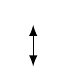
\begin{tikzpicture}
              \path[use as bounding box] (-0.2em, 0) -- (0, 0) -- (0, 1em) -- (-0.2em, 1em) -- cycle;
              \draw[latex-latex] (0, -0.4em) -- (0, 1.1em);
            \end{tikzpicture} &
            \multirow{2}{*}{$\DS \left(\rule[-1.25em]{0pt}{3em}\right.$}
              & \multicolumn{1}{c|}{A}
              & 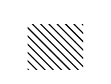
\begin{tikzpicture}
                  \path[use as bounding box] (-1em, 0) rectangle (1em, 1em);
                  \fill[pattern=north west lines] (-1em, -0.5em) rectangle (1em, 1.1em);
                \end{tikzpicture} &
            \multirow{2}{*}{$\DS \left.\rule[-1.25em]{0pt}{3em}\right)$}
          \\\cline{3-4}
            n
            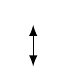
\begin{tikzpicture}
              \path[use as bounding box] (-0.2em, 0) -- (0, 0) -- (0, 1em) -- (-0.2em, 1em) -- cycle;
              \draw[latex-latex] (0, -0.4em) -- (0, 1.1em);
            \end{tikzpicture} &
            & \multicolumn{1}{c|}{O} & \multicolumn{1}{c}{B} &
          \end{array}
        $}}
        \in \setMatrix{\paren{m + n}}{\paren{m + n}}{K}
      $
      に対して
      \begin{align*}
        \det M = \det A \cdot \det B
      \end{align*}
      が成り立つ.
    }
    \thmpar[thm:block-fundamental]{}{
      正方行列
      $\DS
        M =
        \text{\raisebox{0.75em}{$\DS
          \begin{array}{@{}r@{}r@{}c@{}c@{}l@{}}
            &
            & \tikz \draw[latex-latex] (0, 0) -- (2em, 0) node[midway, above] {$m$};
            & \tikz \draw[latex-latex] (0, 0) -- (2em, 0) node[midway, above] {$n$};
            &
          \\
            m
            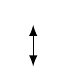
\begin{tikzpicture}
              \path[use as bounding box] (-0.2em, 0) -- (0, 0) -- (0, 1em) -- (-0.2em, 1em) -- cycle;
              \draw[latex-latex] (0, -0.4em) -- (0, 1.1em);
            \end{tikzpicture} &
            \multirow{2}{*}{$\DS \left(\rule[-1.25em]{0pt}{3em}\right.$}
              & \multicolumn{1}{c|}{A} & \multicolumn{1}{c}{B} &
            \multirow{2}{*}{$\DS \left.\rule[-1.25em]{0pt}{3em}\right)$}
          \\\cline{3-4}
            n
            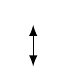
\begin{tikzpicture}
              \path[use as bounding box] (-0.2em, 0) -- (0, 0) -- (0, 1em) -- (-0.2em, 1em) -- cycle;
              \draw[latex-latex] (0, -0.4em) -- (0, 1.1em);
            \end{tikzpicture} &
            & \multicolumn{1}{c|}{C} & \multicolumn{1}{c}{D} &
          \end{array}
        $}}
        \in \setMatrix{\paren{m + n}}{\paren{m + n}}{K}
      $
      に対し,$A$ が正則ならば
      \begin{align*}
        \det M = \det A \cdot \det \paren{D - C A^{-1} B}
      \end{align*}
      が成り立つ.
    }
    \proof{}{
      $A$ が正則であるという仮定より $A$ の逆行列 $A^{-1}$ が一意的に存在し,
      \begin{align*}
        \begin{genmat}{c|c}
          I_{m} & O
        \\\hline
          -C A^{-1} & I_{n}
        \end{genmat}
        \begin{genmat}{c|c}
          A & B
        \\\hline
          C & D
        \end{genmat}
      &=
        \begin{genmat}{c|c}
          A & B
        \\\hline
          O & D - C A^{-1} B
        \end{genmat}
      \end{align*}
      が成り立つ.ここで左辺の行列式は
      \begin{align*}
        \det \paren{
          \begin{genmat}{c|c}
            I_{m} & O
          \\\hline
            -C A^{-1} & I_{n}
          \end{genmat}
          \begin{genmat}{c|c}
            A & B
          \\\hline
            C & D
          \end{genmat}
        }
      &=
        \det
          \begin{genmat}{c|c}
            I_{m} & O
          \\\hline
            -C A^{-1} & I_{n}
          \end{genmat}
        \cdot \det
          \begin{genmat}{c|c}
            A & B
          \\\hline
            C & D
          \end{genmat}
            \holdby{定理~\ref{thm:block-det-ignore-upper-right}}
      \\&=
        1 \cdot \det M
      \\&= \det M
      \end{align*}
      であり,一方右辺の行列式は
      \begin{align*}
        \det
          \begin{genmat}{c|c}
            A & B
          \\\hline
            O & D - C A^{-1} B
          \end{genmat}
        &=
          \det A \cdot \det \paren{D - C A^{-1} B} \holdby{定理~\ref{thm:block-det-ignore-upper-right}}
      \end{align*}
      であるから,以上より $\det M = \det A \cdot \det \paren{D - C A^{-1} B}$ が成り立つ.\qed
    }
    \corpar{}{
      $A \in \setMatrix{n}{m}{K}$,$B \in \setMatrix{m}{n}{K}$ に対し,
      \begin{align*}
        \det \paren{I_{n} + A B} = \det \paren{I_{m} + B A}
      \end{align*}
      が成り立つ.
    }
    \proof{}{
      $\DS
        M \defeq
        \begin{genmat}{c|c}
          I_{m} & -B
        \\\hline
          A & I_{n}
        \end{genmat}
      $
      とおくと
      \begin{align*}
        \det M
        &= \det I_{m} \cdot \det \paren{I_{n} - A I_{m}^{-1} \paren{-B}}
          \holdby{定理~\ref{thm:block-fundamental}}
      \\&= \det \paren{I_{n} + A B}
      \end{align*}
      が成り立ち,一方で
      $\DS
        N \defeq
        \begin{genmat}{c|c}
          I_{n} & A
        \\\hline
          -B & I_{m}
        \end{genmat}
      $
      とおくと同様に
      \begin{align*}
        \det N
        &= \det I_{n} \cdot \paren{I_{m} - \paren{-B} I_{n}^{-1} A}
          \holdby{定理~\ref{thm:block-fundamental}}
      \\&= \det \paren{I_{m} + B A}
      \end{align*}
      が成り立つ.$M$ と $N$ は偶数回の行・列交換により移り合うので $\det M = \det N$ であり,
      ゆえに $\det \paren{I_{n} + A B} = \det \paren{I_{m} + B A}$ である.\qed
    }
  \subsection{餘因子}
    \defpar{餘因子}{
      正方行列 $A \in \setMatrix{n}{n}{K}$ の行列式 $\det A$ を $a_{i j}$ に関する多項式と看なしたときの係数 $\cofactorDelta{A}_{i j}$ を
      $A$ の第 $\seqprn{i, j}$ 成分の\newword{餘因子}と呼ぶ.より形式的には
      \begin{align*}
        \cofactorDelta{A}_{i j} \defeq \paren{-1}^{i + j} \det \submatrix{A}{\Natleq{n} \setmns \setprn{i}}{\Natleq{n} \setmns \setprn{j}}
      \end{align*}
      である.
    }
    \thmpar[thm:laplace-expansion]{Laplace展開}{
      正方行列 $A \in \setMatrix{n}{n}{K}$ と $p, q \in \Natleq{n}$ に対し,以下がそれぞれ成り立つ:
      \begin{align*}
        \det A &= \sum_{j = 1}^{n} A_{p j} \cofactorDelta{A}_{p j}
      \\
        \det A &= \sum_{i = 1}^{n} A_{i q} \cofactorDelta{A}_{i q}
      \end{align*}
    }
    \defpar{餘因子行列}{
      正方行列 $A \in \setMatrix{n}{n}{K}$ に対し,$A$ の\newword{餘因子行列} $\cofactor{A} \in \setMatrix{n}{n}{K}$ を
      \begin{align*}
        \cofactor{A}_{i j} \defeq \cofactorDelta{A}_{j i}
      \end{align*}
      で定める.餘因子を並べたものの転置であることに注意せよ.
    }
    \lempar[lem:cofactor-and-inverse]{餘因子行列と逆行列}{
      正方行列 $A \in \setMatrix{n}{n}{K}$ に対し,$\cofactor{A} A = A \cofactor{A} = \paren{\det A} I_{n}$ が成り立つ.
    }
    \proof{}{
      \begin{align*}
        \paren{\cofactor{A} A}_{i j}
        &= \sum_{k = 1}^{n} \cofactor{A}_{i k} A_{k j}
      \\&= \sum_{k = 1}^{n} A_{k j} \cofactorDelta{A}_{k i}
      \end{align*}
      であるから,
      \begin{itemize}
      \item $i = j$ のとき,
        \begin{align*}
          \paren{\cofactor{A} A}_{i j} = \paren{\cofactor{A} A}_{j j}
          &= \sum_{k = 1}^{n} A_{k j} \cofactorDelta{A}_{k j}
          = \det A
            \holdby{定理~\ref{thm:laplace-expansion}:Laplace展開}
        \end{align*}
      \item $i \neq j$ のとき,
        $B \defeq \coloverwrite{A}{i}{\colvec{A}{j}}$
        とする.すなわち $A$ の第 $i$ 列を第 $j$ 列の各成分で上書きした行列が $B$ である.
        このとき,第 $i$ 列に関するLaplace展開は第 $i$ 列の成分に依存しないから,$\cofactorDelta{B}_{k i} = \cofactorDelta{A}_{k i}$ が成り立つ.
        また $B$ は第 $i$ 列と第 $j$ 列が同一なので $\det B = 0$ であり,これらから
        \begin{align*}
          \paren{\cofactor{A} A}_{i j}
          &= \sum_{k = 1}^{n} A_{k j} \cofactorDelta{A}_{k j}
        \\&= \sum_{k = 1}^{n} A_{k j} \cofactorDelta{B}_{k j}
        \\&= \det B
            \holdby{定理~\ref{thm:laplace-expansion}:Laplace展開}
        \\&= 0
        \end{align*}
        が成り立つ.
      \end{itemize}
      以上より,$\cofactor{A} A = \paren{\det A} I$ である.$A \cofactor{A}$ についても同様.\qed
    }
    \thmpar{Cramerの公式}{
      正則行列 $A \in \setMatrix{n}{n}{K}$,ベクトル $\vecb \in K^{n}$ に対して
      $\vecx \in K^{n}$ が $A \vecx = \vecb$ を満たすならば,各 $i \in \Natleq{n}$ に対して
      \begin{align*}
        \vecx_{i}
        &= \frac{\det \coloverwrite{A}{i}{\vecb}}{\det A}
      \end{align*}
      が成り立つ.
    }
    \proof{}{
      \begin{align*}
        \vecx_{i}
        = \paren{A^{-1} \vecb}_{i}
        &= \sum_{j = 1}^{n} \paren{A^{-1}}_{i j} \vecb_{j}
      \\&= \sum_{j = 1}^{n} \frac{\cofactor{A}_{i j}}{\det A} \vecb_{j}
        \holdby{補題~\ref{lem:cofactor-and-inverse}}
      \\&= \frac{1}{\det A} \sum_{j = 1}^{n} \cofactorDelta{A}_{j i} \vecb_{j}
      \end{align*}
      であり,一方で
      \begin{align*}
        \det \coloverwrite{A}{i}{\vecb}
        &= \sum_{j = 1}^{n} \paren{\coloverwrite{A}{i}{\vecb}}_{i j} \cofactorDelta{\scriptrange{\coloverwrite{A}{i}{\vecb}}}_{j i}
          \holdby{定理~\ref{thm:laplace-expansion}:第 $i$ 列に関するLaplace展開}
      \\&= \sum_{j = 1}^{n} \vecb_{j} \cofactorDelta{A}_{j i}
      \end{align*}
      より $\DS \vecx_{i} = \frac{\det \coloverwrite{A}{i}{\vecb}}{\det A}$ である.\qed
    }
    \thmpar{Binet--Cauchyの公式}{
      $m \leq n$ なる行列 $A \in \setMatrix{m}{n}{K}$,$B \in \setMatrix{n}{m}{K}$ に対して
      \begin{align*}
        \det \paren{A B} &= \sum_{\scriptrange{J \in {\Natleq{n} \choose m}}} \det \colsubmatrix{A}{J} \cdot \det \rowsubmatrix{B}{J}
      \end{align*}
    }
    \proof{}{
      $\DS M \defeq
        \begin{genmat}{c|c}
          I & B
        \\\hline
          A & O
        \end{genmat}
      $ とすると
      \begin{align*}
        \det M
        &= \det I \cdot \det \paren{o - A I^{-1} B}
          \holdby{定理~\ref{thm:block-fundamental}}
      \\&= \det \paren{- A B}
        = \paren{-1}^{m} \det \paren{A B}
      \end{align*}
      が成り立つ.一方,行列式の定義に基づくと
      \begin{align*}
        \det M &= \sum_{\sigma \in \Perm{m + n}} \sgn \sigma \prod_{i = 1}^{m + n} M_{\scriptrange{i \app{\sigma}{i}}}
      \end{align*}
      であり,これを実際に各 $\sigma \in \Perm{m + n}$ について和をとって求めてみる.
      $\DS \prod_{i = 1}^{m + n} M_{\scriptrange{i \app{\sigma}{i}}} \neq 0$ なる $\sigma \in \Perm{m + n}$ についてのみ考えればよい.
      このような $\sigma$ に対し,$\DS J \in {\Natleq{n} \choose m}$ が存在して $\forallin{j}{\Natleq{n} \setmns J}{\app{\sigma}{j} = j}$
      を満たす.\REMAINS \NEEDPICTURE
    }
  \subsection{階数}
    \defpar{行列の階数}{
      簡単のためここでは線型写像と行列を同一視することにすると,
      $\funcdoms{A}{V}{U}$ に対して $A$ の\newword{階数}は
      $\rank A \defeq \dim \paren{\Img A} = \dim V - \dim \paren{\Ker A}$ で定められる.
      行列の直観としては「掃き出した後に対角に並ぶ非零成分の個数」である.
    }
    \lempar[lem:rank-fundamental-ineq]{}{
      以下がそれぞれ成り立つ:
      \begin{thmenum}
      \thmenumitem\label{lem:rank-fundamental-ineq|1}
        $\forallin{A}{\setMatrix{m}{l}{K}}{\forallin{B}{\setMatrix{l}{n}{K}}{
          \rank \paren{A B} \leq \min \setprn{\rank A, \rank B}}}$
      \thmenumitem\label{lem:rank-fundamental-ineq|2}
        正則行列 $S \in \setMatrix{m}{m}{K}$,$T \in \setMatrix{l}{l}{K}$ に対して
        $\rank A = \rank \paren{S A T}$
      \thmenumitem\label{lem:rank-fundamental-ineq|3}
        $\forallin{A|B}{\setMatrix{m}{n}{K}}{
          \rank \paren{A + B} \leq \rank A + \rank B}$
      \end{thmenum}
    }
    \proof{}{
      \subproof{\ref{lem:rank-fundamental-ineq|1}}{
        $\Img \paren{A B} \subseteq \Img A$ より $\rank \paren{A B} \leq \rank A$.また,
        $\rank \paren{A B} = \rank \trsps{\paren{A B}} = \rank \paren{\trsps{B} \trsps{A}} \leq \rank \trsps{B} = \rank B$.\qed
      }
      \subproof{\ref{lem:rank-fundamental-ineq|2}}{
        \ref{lem:rank-fundamental-ineq|1}より $\rank \paren{S A T} \leq \rank \paren{A}$,
        一方で同様に $\rank A = \rank \paren{S^{-1} S A T T^{-1}} \leq \rank \paren{S A T}$ が成り立ち,
        $\rank A = \rank \paren{S A T}$.\qed
      }
      \subproof{\ref{lem:rank-fundamental-ineq|3}}{
        掃き出しにより
        \begin{align*}
          \rank
          \begin{genmat}{c|c}
            I & A
          \\\hline
            -I & B
          \end{genmat}
        &=
          \rank
          \begin{genmat}{c|c}
            I & A
          \\\hline
            O & A + B
          \end{genmat}
        = m + \rank \paren{A + B}
        \end{align*}
        \REMAINS \NEEDPICTURE
      }
    }
  \subsection{正定値性}
    \defpar{正定値性,半正定値性}{
      正方行列 $A \in \setMatrix{n}{n}{K}$ が $\forallin{\vecx}{K^{n} \setmns \setprn{\veczero}}{\trsps{\vecx} A \vecx > 0}$ を満たすとき,
      $A$ は\newword{正定値}であるといい,また $A$ が $\forallin{\vecx}{K^{n}}{\trsps{\vecx} A \vecx \geq 0}$ を満たすとき,
      $A$ は\newword{半正定値}であるという.
    }
    \lempar[lem:definite-sym-positive-det]{}{
      正方行列 $A \in \setMatrix{n}{n}{K}$ に対し,$A$ が正定値対称ならば $\det A > 0$ である.
    }
    \proof{}{
      $A$ の大きさ $n$ に関する帰納法による.
      \begin{itemize}
      \item $n = 1$ のときは明らか.
      \item $n = k\geq 2$ のとき,
        $\DS A =
          \begin{genmat}{c|c}
            a & \trsps{\vecc}
          \\\hline
            \vecc & \expandHV{D}
          \end{genmat}
        $
        とおくと,$A$ が正定値である仮定より
        \begin{align*}
          0
          &<
            \trsps{\vecsglone{1}} A \vecsglone{1}
        \\&=
            \begin{genmat}{c|c}
              1 & \expandH{\trsps{\veczero}}
            \end{genmat}
            \begin{genmat}{c|c}
              a & \trsps{\vecc}
            \\\hline
              \vecc & \expandHV{D}
            \end{genmat}
            \begin{genmat}{c}
              1
            \\\hline
              \expandV{\veczero}
            \end{genmat}
          = a
        \end{align*}
        であるから $a > 0$.また定理~\ref{thm:block-fundamental}より
        $\DS \det A = a \cdot \det \paren{D - \frac{1}{a} \vecc \trsps{\vecc}}$ が成り立つ.ここで
        \begin{align*}
          A' \defeq
          \begin{genmat}{c|c}
            a & \trsps{\veczero}
          \\\hline
            \veczero & \DS\expandHV{D - \frac{1}{a} \vecc \trsps{\vecc}}
          \end{genmat}
        \end{align*}
        とすると $\det A = \det A'$.このとき
        \begin{align*}
          \begin{genmat}{c|c}
            y & \expandH{\trsps{\vecz}}
          \end{genmat}
          \begin{genmat}{c|c}
            a & \trsps{\veczero}
          \\\hline
            \veczero & \DS\expandHV{D - \frac{1}{a} \vecc \trsps{\vecc}}
          \end{genmat}
          \begin{genmat}{c}
            y
          \\\hline
            \expandV{\vecz}
          \end{genmat}
          &= a y^{2} + \trsps{\vecz} D \vecz - \frac{1}{a} \paren{\trsps{\vecc} \vecz}^{2}
        \\
          \begin{genmat}{c|c}
            y & \expandH{\trsps{\vecz}}
          \end{genmat}
          \begin{genmat}{c|c}
            a & \trsps{\vecc}
          \\\hline
            \vecc & \expandHV{D}
          \end{genmat}
          \begin{genmat}{c}
            y
          \\\hline
            \expandV{\vecz}
          \end{genmat}
          &= a y^{2} + 2 y \trsps{\vecc} \vecz + \trsps{\vecz} D \vecz
        \end{align*}
        \REMAINS
      \end{itemize}
    }
    \thmpar{}{
      対称行列 $A \in \setMatrix{n}{n}{K}$ に対し,$A$ が正定値であることと $A$ の任意の首座小行列式が正であることは同値.
    }
    \thmpar[thm:definite-sym-inverse]{}{
      行列 $A \in \setMatrix{n}{n}{K}$ に対し,$A$ が正定値対称ならば $A^{-1}$ も正定値対称.
    }
    \proof{}{
      $A$ を正定値対称とすると,$A$ は正則であるから逆行列 $A^{-1}$ をもつ.
      $\vecx \in K^{m} \setmns \setprn{\veczero}$ とすると
      \begin{align*}
        \trsps{\vecx} A \vecx
        &= \trsps{\vecx} A^{-1} A A^{-1} \vecx
      \\&= \trsps{\paren{A \vecx}} A \paren{A \vecx} > 0
          \holdby{$A$ は正定値}
      \end{align*}
      であるから,$A^{-1}$ は正定値.対称性は
      $\trsps{\paren{A^{-1}}} = \paren{\trsps{A}}^{-1} = A^{-1}$
      より明らか.\qed
    }
    \thmpar{}{
      行列 $A \in \setMatrix{n}{n}{K}$ が正定値対称ならば,$\DS \det A \leq \prod_{i = 1}^{n} A_{i i}$ が成り立つ.
    }
    \proof{}{
      $A$ の大きさ $n$ に関する帰納法による.
      \begin{itemize}
      \item $n = 1$ のときは $\det A = A_{1 1}$ より自明.
      \item $n \geq 2$ のとき,
        $\DS A =
          \begin{genmat}{c|c}
            a & \trsps{\vecc}
          \\\hline
            \vecc & \expandHV{D}
          \end{genmat}
        $
        とする.仮に $D$ が正定値でないとすると,或る $\vecx \in K^{n - 1} \setmns \setprn{\veczero}$ が存在して
        $\trsps{\vecx} D \vecx \leq 0$ を満たすが,この $\vecx$ を用いると
        \begin{align*}
          \begin{genmat}{c}
            0
          \\\hline
            \expandV{\vecx}
          \end{genmat}
          A
          \begin{genmat}{c}
            0
          \\\hline
            \expandV{\vecx}
          \end{genmat}
          &=
            \trsps{\vecx} D \vecx
          < 0
        \end{align*}
        より $A$ の正定値性に反するから $D$ は正定値.よって $D$ は正則であり,
        \begin{align*}
          \det A
          = \det
            \begin{genmat}{c|c}
              a & \trsps{\vecc}
            \\\hline
              \vecc & \expandHV{D}            
            \end{genmat}
          &= \det
            \begin{genmat}{c|c}
              \expandHV{D} & \vecc
            \\\hline
              \trsps{\vecc} & a
            \end{genmat}
          \holdby{$1$ 回の行交換と $1$ 回の列交換}
        \\&= \det D \cdot \det \paren{a - \trsps{\vecc} D^{-1} \vecc}
          \holdby{定理~\ref{thm:block-fundamental}}
        \end{align*}
        が成り立つ.定理~\ref{thm:definite-sym-inverse}より $D^{-1}$ も正定値対称であるから
        $\trsps{\vecc} D^{-1} \vecc \geq 0$,また定理~\ref{lem:definite-sym-positive-det}より $\det D > 0$ が成り立ち,よって
        $\det A = \det D \cdot \paren{a - \trsps{\vecc} D^{-1} \vecc} \leq \det D \cdot a$ である.
        ここで帰納法の仮定より $\DS D \leq \prod_{i = 1}^{n - 1} D_{i i} = \prod_{i = 2}^{n} A_{i i}$ であり,ゆえに
        \begin{align*}
          \det A
          \leq \det D \cdot a
          \leq \paren{\prod_{i = 2}^{n} A_{i i}} \cdot a
          &= \paren{\prod_{i = 2}^{n} A_{i i}} \cdot A_{1 1}
          = \prod_{i = 1}^{n} A_{i i}
        \end{align*}
        が成り立つ.
      \end{itemize}
      以上より,$\DS \det A \leq \prod_{i = 1}^{n} A_{i i}$ が成り立つ.\qed
    }
  \subsection{固有値と固有ベクトル}
    \defpar{共軛転置行列,正規行列,ユニタリ行列,Hermite行列}{
      行列 $A \in \setMatrix{m}{n}{\setC}$ に対し,$\paren{\conjtrsps{A}}_{i j} \defeq \conj{A_{j i}}$ で
      定義される $\conjtrsps{A} \in \setMatrix{n}{m}{\setC}$ を $A$ の\newword{共軛転置行列}と呼ぶ.
      $A \conjtrsps{A} = \conjtrsps{A} A$ なる正方行列 $A$ を\newword{正規行列},
      $A \conjtrsps{A} = I$ なる正方行列 $A$ を\newword{ユニタリ行列},
      $A = \conjtrsps{A}$ なる正方行列 $A$ を\newword{Hermite行列}と呼ぶ.
    }
\end{document}